\section{ASIC Design Flow}

The digital implementation of Desing includes the following steps

\begin{figure}[h]
    \centering
    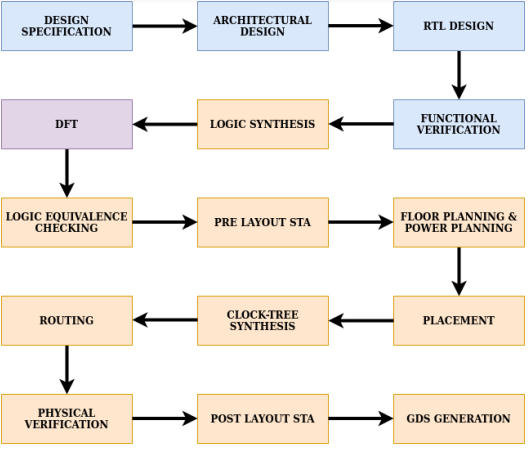
\includegraphics[width = 0.9\linewidth]{./Theory/ASIC.png}
    \caption{ASIC Design Flow\cite{Sunny}}
    %\label{fig:Intro:flow}
\end{figure}
\begin{enumerate}
    \item Design Specification: Design Specification is based on the application provided by the consumer to the designer. This majorly includes the performance requirements under the Budget of area and power.

    \item Architecture Design: the Architecture Designer create the architectural view of microarchitecture and protocols from the design specification as per the requirement.

    \item RTL Design: The RTL designer codes the microarchitecture under the specification using Hih Level Description Langauge. This includes the behavioral and data flow modeling of Design.

    \item Functional Verification: The functional Verification is the essential part where the design specifications, i.e., the architecture integrations and protocols, are verified over one head. The RTL designer and verification team work resemblance for Architecture demands as per the Design Specification. The process here would include the functional part, i.e., i.ee. They matched the requirements without considering the area, power, or timing conditions.

    \item Logical Synthesis: The logical Synthesis is the process of RTL code to map with the Standard cells to form a gate-level netlist. Foundries provide the standard cells. The performance is decided by the technology nodes used to synthesize the RTL, and the optimum value is synthesis is done as per the timing and power budget of the Design.

    \item Design for Test: The testability done after synthesis that would be used after manufacturing the Design. This step includes the generation of test vectors to find the Design's testability.

    \item Logical Equivilance Checking: The process of logical equivalence of RTL with the gate level in the stage of pre and post-PnR.The Gate level simulation of generated netlist would delay the process. Therefore, the Logical Equivalence is used as an alternative where reduced boolean and their equivalence is checked.

    \item Pre-Layout STA: After Logical equivalence, the Timing analysis is as per the design requirement. This would be the end of Front end Design.

    \item Floor planning and Power Planning: The Aim is to define the Aspect ratio and Utilization Area of Design over the chip. This step includes Partitioning of the Design, Macro Placements, and Power planning of the Design.

    \item Placements: The Netlist generated by the Synthesis tool is used and placed under the constraints of floor planning. Filler Cells are filled to ensure that all power nets are connected. It does take place in stages
    \begin{itemize}
        \item Pre Placement Optimization contains the downsizing of cells
        \item In Placement: performs cell bypassing, gate duplications 
        \item Post Placement optimization for Timing violations based on the routings
    \end{itemize}

    \item Clock tree Synthesis(CTS): CTS is to minimize the sket and insertion of delay. Clock Tree analyzed the structures under timing and power constraints.

    \item Routing: This step is interconnecting the Macros. There are two kinds of routing:
    \begin{itemize}
    \item  Global Routing: The routing is loose routed is generated to estimate the delay for final routing
    \item Detail routing: The actual geometry layout of the net is done, including the substantial delay with optimization for timing, DRC, and Antenna effect is done.
    \end{itemize}
    
    \item Physical Verification: The physical verification is done to check the foundry based Rules for proper functioning
    \begin{itemize}
    \item DRC: Design as per the required rules given by Foundry
    \item LVS: Layout versus netlist generated by synthesis tools verification
    \item ARC: Design to flag any open-ended track/arc primitive, or open-ended track / arc that is terminated with a via checks
    \end{itemize}

    \item RC Extractions and Post Layout STA: extraction is done, and final Post Layout Timing Is verified with interconnects delas

    \item GDSI generation: Final binary file representing the planar geometric shapes and other information that foundries would use for tape-out
\end{enumerate}